The frame M is a counterclockwise rotation of the global frame G by $\frac{\pi}{3}$ radians.

Draw the basis vectors for frame G and frame M.

\begin{solution}\
\begin{center}
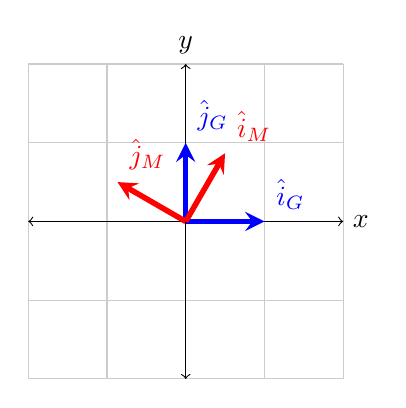
\begin{tikzpicture}
  \draw[thin,gray!40] (-2,-2) grid (2,2);
  \draw[<->] (-2,0)--(2,0) node[right]{$x$};
  \draw[<->] (0,-2)--(0,2) node[above]{$y$};
  \draw[line width=2pt,blue,-stealth](0,0)--(1,0) node[anchor=south west]{$\boldsymbol{\hat{i}}_G$};
  \draw[line width=2pt,blue,-stealth](0,0)--(0,1) node[anchor=south west]{$\boldsymbol{\hat{j}}_G$};
  \draw[line width=2pt,red,-stealth](0,0)--(0.5, 0.866) node[anchor=south west]{$\boldsymbol{\hat{i}}_M$};
  \draw[line width=2pt,red,-stealth](0,0)--(-0.866, 0.5) node[anchor=south west]{$\boldsymbol{\hat{j}}_M$};
\end{tikzpicture}
\end{center}
\end{solution}